\chapter{Re-engineer MediaSense}
\section{Problem Explication}
The explicate problem step in Design Science \cite{johannesson2012design} is to formulate precisely the initial problem and investigate its underlying causes. To define the problem as precisely as possible, a scenario will be defined. The problem was split into several sub-problems. As mentioned before the research method for explicating the problem is a document study of previous publications regarding distributed Internet of Things middleware, a document study of the source code for MediaSense and interviews with the lead developer of MediaSense. 

%\subsection{Research Question}
As the authors discuss in \cite{johannesson2012design} a research question was formulated to form the basis of the problem explication. For the problem explication part of the project the research questions is the following: 

\begin{quotation}
What are the major issues with current implementations of distributed Internet of Things middleware which make them unable to realize the Internet of Things vision?
\end{quotation}

%\subsection{Method Application}
To explicate the problem a document study of previous publications regarding distributed Internet of Things and middleware for it was done. Some of the publications regarding MediaSense were provided by the stakeholder \cite{TheMediaSenseFramework}, \cite{Kanter539187}, \cite{Walters413794}. These provide background on Internet of Things, what MediaSense is and how it works theoretically. Publications about Internet of Things and the surrounding theories were found by searching IEEE Xplore, ACM Digital library and Google Scholar. The main search queries used were \emph{Internet of Things}, \emph{Internet of Things middleware}, \emph{Internet of Things centralized} and \emph{Internet of Things decentralized}. Because the concept Internet of Things is a popular research area, a lot of articles was found. Publications was selected by reading the abstract to see if the publication were able to expand the knowledge base for the problem, searches for keywords were done and ranking publications after number of citations was done to narrow down the search result. 

After getting a grasp of the current state of Internet of Things middleware unstructured interviews were conducted with the stakeholder and main contributor to the MediaSense platform. This respondent has a lot of experience with distributed computing and a good understanding of how Internet of Things middlewares works, therefore this respondent was the best person to interview. The interviews were conducted in an informal manner in both the stakeholders office and in a conference room with access to a whiteboard. No recording or notes were done for the interviews thus availed both authors to be active in the interviews and discussions could be done without thinking of recording or taking notes. These interviews were conducted iteratively and in parallel with a document study of the existing source code of MediaSense. This document study yielded questions for upcoming interviews and the interviews in turn gave more information about the inner workings of Internet of Things middlewares and how to proceed the study of MediaSense's source code.

Interviews began with trying to discover the problematics of the chosen Internet of Things middleware. The stakeholder first presented a problem that had been identified with MediaSense, a large resource overhead when running multiple applications. The first set of interview questions served to fill the gaps that documentation normally would. The questions aimed to explore how MediaSense worked and to get a broader knowledge base. After studying the source code and getting an understanding of the architecture, the interview questions explored certain modules functionality and how they worked. When the interviewee responded to the questions in an uncertain manner, the follow up questions were formulated to ascertain how they were supposed to work or how it was intended they should work.

After the application of methods used to explicate the problem an analysis was done on the result from the interviews and the document study. This was done by putting together the result from the interviews and the knowledge that was built when the document study of code was done. By using the answers from the interviews and reproducing the problems mentioned by the respondent on a developer instance of MediaSense, the problem was clearer from a technical view.

\section{Results And Analysis}
The following scenario describes a use case scenario of an Internet of Things platform.

\subsection{Scenario}
Johan is CEO for a company in Stockholm. He is always on the move from meetings with his co-workers at work and to his daughter's football practice after work. His apartment is equipped with broadband and he has a Raspberry Pi computer connected to the Internet through a router. This Raspberry Pi is working as an information hub for Johan. The computer is running a distributed Internet of Things middleware and has 20 application installed. Johan has bought a new temperature regulator for his apartment. This regulator comes with an application that can be installed on his information hub. The temperature regulator is context-aware, it gets GPS information from Johans mobile phone and regulates the temperature in his apartment according to this. When he leaves home every morning the heating in the apartment turns down. At work Johan receive notifications to leave for meetings based on where the meetings are and how long it will take him to get there. When Johan leaves work his car's navigation system checks with his calendar if he has anything on his schedule, discovers his daughter has football practice and plots a course to the practice to pick her up. Johan's mobile phone alerts his heating regulator as he approaches his home and the heating is turned back on. Another application is connected to a thermometer by Johan's house and collects information about the temperature outdoors and adjusts the heating of according to this information.

\subsection{Define problem}
Distributed Internet of Things middlewares are resource heavy, which makes them inefficient to run on ubiquitous devices. Centralized Internet of Things middleware can solve this problem, but centralized approaches are more vulnerable and it can not be guaranteed that the server is always up and ready to respond to clients requests. Therefore, a distributed Internet of Things middleware needs to be redesigned to reduce the resource footprint. The chosen middleware for redesign is MediaSense. MediaSense is being developed by researchers at the Department of Computer and System Sciences at Stockholm University and is open source. 

After the interviews and document study of the source code of MediaSense the main reason for the resource overhead was identified. MediaSense in its present form makes it necessary to run the platform once for every application. Every application running on a device needs its own instance of the middleware. This makes it necessary to run a middleware for every application running on a device, which is the main reason of the resource overhead. 

\begin{figure}[h!]
		\centering
    	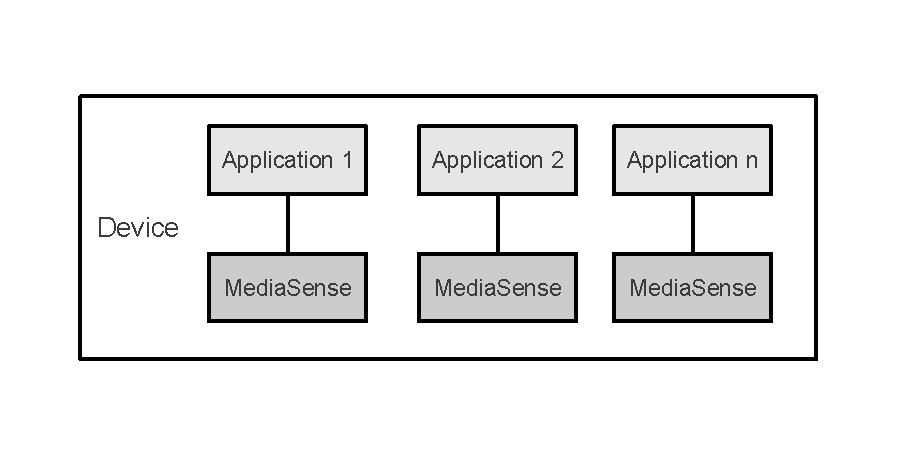
\includegraphics[scale=0.75]{part_4/result_and_analysis/mediasense_arch_old.pdf}
		\caption{The current state of the Mediasense platform showing how every application need its own instance of MediaSense.} 
\end{figure}

A sub-problem to the multiple middleware instances is that every instance need its own port for communicating. Because MediaSense is communicating over IP every instance needs its own port open. This means that a user needs to open new ports on the router and firewall for every application running on the device. When several instances of MediaSense is running on a device the network traffic increases, more processing power is used and more memory is used. 

\subsection{Motivation}
To make the scenario presented above possible an Internet of Things middleware it is needed to facilitate the communication between devices. Because the devices used in the scenario are mobile this middleware needs to be resource efficient. The devices need to handle a multitude of applications. Given the current state of MediaSense, the scenario will not be possible because of the resource overhead. To make the Internet of Things concept possible on ubiquitous devices this resource overhead must be dealt with.

\subsection{Analysis Of Problem}
With distributed Internet of Things middlewares every instance of the middleware is both a \emph{server} and a \emph{client}. Every instance of the middleware have its own network layer and database layer for storing context information. In a centralized middleware the server functionality can be moved to a centralized computer and therefore centralized middleware are more lightweight. This is one of the reasons distributed Internet of Things middleware are resource heavy. 

To reduce the resource overhead it is prefered to change the architecture of MediaSense. Changing the architecture so that only one shared instance of MediaSense is running can reduce the resource used on a device.  As shown in figure the desired architecture of MediaSense MediaSense will be run as an underlying  \emph{daemon} and every application needing the services from the platform can use the daemon. This also solves the subproblem with multiple network layers on one device. Devices only need one open port on router or firewall to communicate with other nodes in the network.  

\begin{figure}[h!]
	\centering
    	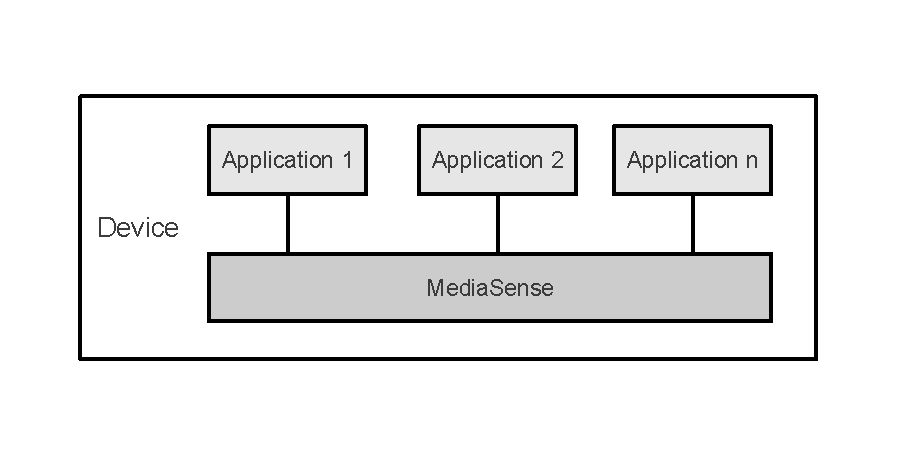
\includegraphics[scale=0.75]{part_4/result_and_analysis/mediasense_arch_new.pdf}
    	\centering
		\caption{The desired state of the Mediasense platform.} 
\end{figure}

